\documentclass[article]{jss}

\usepackage{orcidlink,thumbpdf,lmodern}
\usepackage{amssymb,amsmath,amsthm,mathtools,bm}
\usepackage{upquote}

\usepackage{microtype}
\UseMicrotypeSet[protrusion]{basicmath} % disable protrusion for tt fonts

\usepackage{booktabs}
\usepackage{caption}
\usepackage{subcaption}
\usepackage{siunitx}

\usepackage[linesnumbered,vlined,ruled]{algorithm2e}

\usepackage{enumitem}

\usepackage[capitalize,noabbrev]{cleveref}
\usepackage{crossreftools}
\pdfstringdefDisableCommands{%
  \let\Cref\crtCref
  \let\cref\crtcref
}

\usepackage{todonotes}

% Workaround for Gin settings
\makeatletter
\let\natwidth\Gin@nat@width
\makeatother

\DeclareMathOperator*{\minimize}{minimize}
\newcommand{\link}{g}
\newcommand{\ilink}{g^{-1}}
% \newcommand{\link}[1]{\expandafter\newcommand\csname #1\endcsname[1]{#1(##1)}}


% setup url command for hyperref
\newcommand{\myurl}[1]{\href{https://#1}{\nolinkurl{#1}}}

\author{Johan Larsson~\orcidlink{0000-0002-4029-5945}\\University of Copenhagen
   \And Second Author\\Plus Affiliation}
\Plainauthor{}

\title{Efficient Solvers for SLOPE in \proglang{R}, \proglang{Python}, \proglang{Julia}, and \proglang{C++}}
\Plaintitle{Efficient Solvers for SLOPE in R, Python, Julia, and C++}
\Shorttitle{Efficient Solvers for SLOPE}

\Abstract{
  We present a collection of packages in \proglang{R}, \proglang{Python},
  \proglang{Julia}, and \proglang{C++} to efficiently solve the full
  regularization path for Sorted L-One Penalized Estimation (SLOPE) in
  \proglang{R}, \proglang{Python}, \proglang{Julia}, and \proglang{C++}.
  The packages feature a new and improved implementation of the 
  hybrid coordinate descent algorithm for solving SLOPE, which
  features improved and robust convergence properties.
}

\Keywords{SLOPE, OWL, regularization, generalized linear models, \proglang{R}, \proglang{Python}, \proglang{Julia}, \proglang{C++}}
\Plainkeywords{SLOPE, OWL, regularization, generalized linear models, R, Python, C++}

\Address{
  Johan Larsson\\
  Department of Mathematical Sciences\\
  Faculty of Science\\
  University of Copenhagen\\
  Universitetsparken 5\\
  2100 København Ø, Denmark\\
  E-mail: \email{jolars@posteo.com}\\
  URL: \url{https://jolars.co/}
}

\begin{document}

\section{Introduction}

Sorted L-One Penalized Estimation
(SLOPE)~\citep{bogdan2013,zeng2014,bogdan2015} is a type of
regularized regression that consists of the following convex optimization problem:
\begin{equation}
  \label{eq:slope}
  \minimize_{\beta_0 \in \mathbb{R},\beta \in \mathbb{R}^p}
  \Big(
  P(\beta_0,\beta)
  = F(\beta_0, \beta) + \alpha J_{\lambda}(\beta)
  \Big)
\end{equation}
where \(P\) is the primal problem, \(F\) is the loss function, \(\alpha\) a parameter
that controls the strength of regularization, and \(\lambda\) a non-increasing sequence of penalty weights. \(J\) is the
\emph{sorted $\ell_1$ norm}, defined as
\begin{equation}
  \label{eq:sl1}
  J_{\lambda}(\beta) = \sum_{j=1}^p \lambda_j |\beta_{(j)}|, \quad
  \text{where}\quad |\beta_{(1)}| \geq |\beta_{(2)}| \geq \ldots \geq
  |\beta_{(p)}|.
\end{equation}

We will assume that \(F\) takes the following form:
\[
  F(\beta_0, \beta) = \frac{1}{n} \sum_{i=1}^n f(y_i, \beta_0 + x_i^\intercal \beta),
\]
where \(f\) is a convex function, \(y_i\) is the response variable, and
\(x_i\) is the \(i\)th row of the design matrix.

We let \((\hat{\beta}_0, \hat{\beta})\) denote a solution to the problem in \Cref{eq:slope}
and take \(X\) to be the \(n \times p\) design matrix and \(Y\) the
\(n \times m\) response matrix,\footnote{For our case, \(m = 1\) unless
  the model is multinomial logistic regression.} using the convention
of denoting a row of a matrix \(X\) as \(x_i\) and a column as \(x_j\).

SLOPE is a generalization of OSCAR (octagonal shrinkage and clustering
algorithm for regression)~\citep{bondell2008}, which is attained by
setting \(\lambda\) to be a linear sequence, which is typically parameterized as
\(\lambda_j = \theta_1 + \theta_2(p - j)\),\footnote{We have used \(\theta_1,\theta_2\) in place of
  \(\lambda_1,\lambda_2\), used in \citet{bondell2008}, to avoid abusing notation.} where \(\theta_1, \theta_2
\geq 0\)~\citep{figueiredo2014}. It is also a special case of
the lasso~\citep{santosa1986,donoho1994,donoho1995,tibshirani1996},
which is obtained by taking a constant \(\lambda\).

% SLOPE is a flexible method, which comes from the fact that the
% \(\lambda\) sequence can be chosen in many different ways (including
% the two mentioned above).

% net~\citep{zou2005}, the SCAD (smoothly clipped absolute deviation)
% penalty~\citep{fan2001}, and the MCP~(minimax concave
% penalty)~\citep{zhang2010} for sparse regression.

A special property of SLOPE is that it can clusters coefficients by
setting them to the same magnitude~\citep{figueiredo2016,bogdan2022}. This is a natural
consequence of the sorted \(\ell_1\) norm, stemming from the fact that
the contribution to the norm of a given coefficient increases disproportionally if it
changes order.

SLOPE is a convex but non-smooth optimization problem. But since the
pool-adjacent-violators algorithm~(PAVA)~\citep{barlow1972} can be used to
efficiently\footnote{At an average \(p \log p\) rate, due to the limiting
  sorting operation.} compute the proximal operator of the sorted \(\ell_1\)
norm, it is possible to use a wide range of proximal algorithms, such
as proximal gradient descent, to solve SLOPE. This also includes accelerated
methods such as FISTA~\citep{beck2009}, which is used in the original
implementation of SLOPE by \citet{bogdan2015}. Other possibilities include
proximal Newton~\citep{lee2014} and the alternating direction method of
multipliers (ADMM) method~\citep{boyd2010}.

Although all of aforementioned methods are important and typically robust, they
have for related problems such as the lasso and elastic net been shown to be
inferior to coordinate descent methods~\citep{friedman2007,friedman2010}. For
SLOPE, however, coordinate descent cannot be used directly since the sorted
\(\ell_1\) norm is not separable. This problem was, however, solved by
\citet{larsson2023}, who invented a hybrid combination of proximal gradient and
coordinate descent. The algorithm alternates between full gradient descent
steps and coordinate descent on current cluster structure to achieve robust and
fast convergence.

In this paper, we present a collection of packages (in \proglang{R},
\proglang{Python}, \proglang{Julia}, and \proglang{C++}) that implement an
improved version of this algorithm, which makes this fast and robust algorithm
available to a wide audience.

\subsection{Outline of the paper}

In \Cref{sec:math-details}, we introduce the statistical problem that our
packages solve, namely generalized linear models (GLMs) regularized with the sorted
\(\ell_1\) norm (SLOPE)\footnote{SLOPE is sometimes used only as the procedure
  that uses quadratic loss, but here we adopt a more general terminology and
  let SLOPE be defined for any loss function.}, and provide a brief overview of
the mathematical properties of GLMs and the particular properties of SLOPE.
We also discuss the optimization problem and describe the hybrid
coordinate descent algorithm we use for solving SLOPE.

In \Cref{sec:implementation-details}, we provide a detailed overview of the
software implementations, focusing on technical aspects such as
memory management, parallelization, and convergence criteria.

\section{Mathematical details}\label{sec:math-details}

\subsection{Generalized linear models}
\label{sec:glm}

In this section we provide a brief overview of generalized linear models (GLMs)
and introduce the notation used in the following sections. We fist of all,
we remind the reader that our loss function is defined as
\[
  F(\beta_0, \beta) = \frac{1}{n} \sum_{i=1}^n f(y_i, \eta_i),
\]
letting \(\eta_i = x_i^\intercal \beta + \beta_0\) be the
linear predictor.

In a generalized linear model, the response variable \(y_i\) is modelled
as a random variable from an exponential family, and is assumed to depend
conditionally on the linear predictor \(\eta_i\) through
\[
  \E(y_i \mid \eta_i) = \ilink(\eta_i),
\]
whee \(\ilink\) is the inverse link function.

To estimate the parameters of the model, \(\beta_0, \beta\), we form a loss
function from the negative log-likelihood of the target distribution, modeling
its mean parameter through the inverse link funktion applied to the linear
predictor. A special attribute of resulting loss function is that its partial
derivative with respect to \(\eta\) is the
\emph{generalized residual}
\[
  \frac{\partial}{\partial \eta_i} f(y_i, \eta_i) = \ilink(\eta_i) - y_i = r_i.
\]
As a consequence, the gradient of the loss function with respect to \(\beta_0\)
and \(\beta\) can be expressed as
\[
  \frac{\partial}{\partial \beta_j} F(\beta_0,\beta)
  = \frac{1}{n} \sum_{i=1}^n x_{ij} \frac{\partial}{\partial \eta_i} f(y_i, \eta_i)
  = \frac{1}{n} \sum_{i=1}^n x_{ij} r_i
\]

\begin{table}[t!]
  \centering
  \label{tab:glm}
  \begin{tabular}{lccc}
    \toprule
    Model       & \(f(y, \eta)\)                                                                                       & \(\link(\mu)\)                            & \(\ilink(\eta)\)                                       \\
    \midrule
    Gaussian    & \(\frac{1}{2}(y - \eta)^2\)                                                                          & \(\mu\)                                   & \(\eta\)                                               \\
    \addlinespace
    Binomial    & \(\log(1 + e^\eta) - \eta y\)                                                                        & \(\log \left(\frac{\mu}{1 - \mu}\right)\) & \(\frac{e^\eta}{1 + e^\eta}\)                          \\
    \addlinespace
    Poisson     & \(e^\eta - \eta y\)                                                                                  & \(\log(\mu)\)                             & \(e^\eta\)                                             \\
    \addlinespace
    Multinomial & \(\sum_{k=1}^{m-1}\left( \log \left( 1 +  \sum_{j=1}^{m-1} e^{\eta_j}\right) - y_k \eta_k  \right)\) & \(\log\left(\frac{\mu}{1 - \mu}\right) \) & \(\frac{\exp(\eta)}{1 + \sum_{j=1}^{m-1} e^{\eta_j}}\) \\
    \bottomrule
  \end{tabular}
  \caption{Loss functions, link functions, and inverse link functions for
    generalized linear models in the SLOPE package. Note that in the case of
    multinomial logistic regression, the input vector-valued, and we allow
    \(\log\) and \(\exp\) to be overloaded to apply element-wise in these cases.
  }
\end{table}

A particular case of interest is the multinomial logistic regression model.
Many implementations of regularized multinomial logistic regression models, such
as those by \citet{friedman2010} and \citet{fercoq2015} use the \emph{redundant}
\(m\)-class formulation. Here, however, we have opted to use the non-redundant
formulation of the loss function, with the last class serving as the reference
category. This choice complicates notation slightly and leads to a more
complicated formulation for the dual problem. For SLOPE, however, this is a
more natural choice since it generalizes to the binary case as well (in which
the last class is also implicit). SLOPE needs a \(\lambda\) sequence of length
\(mp\), so the loss function for the multinomial case would not be equivalent
to the binary case if we used the redundant formulation. Furthermore, the
redundant formulation is not estimable in the absence of regularization, which
is not the case for the non-redundant formulation. This fact also means that a
coordinate descent algorithm needs bounds checks to handle the parameter
ambiguity~\citep{friedman2010}. This is not especially difficult to implement
for the lasso, but is more complicated in the case of SLOPE since rows of the
coefficient matrix cannot be arbitrarily shifted since that would alter the
overall cluster structure.

\subsection{Hybrid Algorithm}

The primary algorithm of the \pkg{SLOPE} packages is the hybrid
coordinate descent algorithm by \citet{larsson2023}. Since it is described in
detail there, we will only summarize its key points here.

The basic idea of the algorithm is to perform the coordinate descent updates on
the cluster coefficients, rather than directly on the clusters. In effect, we fix the
current cluster and update all coefficients belong to it in a single step.
On its own, this algorithm is not guaranteed to converge since it can only
reorder or merge clusters. In order to guarantee converge, the algorithm must
therefore be combined with proximal gradient descent steps. These steps
are able to split the clusters, which eventually means that the full
algorithm converges to the correct clusters and global minimum.

\begin{algorithm}[t]
  \caption{The Hybrid coordinate descent algorithm for generalized linear models, using
    the IRLS where weights \(w\) and a working response \(z\) are computed after
    a proximal gradient descent step.}
  \label{alg:hybrid}
  \SetKwInOut{Input}{input}
  \SetKwComment{tcc}{$\triangleright$ }{}
  \SetCommentSty{textit}

  \Input{%
    \(X \in \mathbb{R}^{n\times p}\),
    \(y\in \mathbb{R}^n\),
    \(\lambda \in \{\mathbb{R}^p : \lambda_1 \geq \lambda_2 \geq \cdots > 0\}\),
    \(v \in \mathbb{N}\)
  }

  \Repeat{\(P(\beta_0, \beta) - D(\theta) \leq \varepsilon|P(\beta_0, \beta)|\)}{

    Set \(t\) with backtracking line search\;

    \(\beta \gets \beta - t \nabla F(\beta_0, \beta)\)\; \label{alg:hybrid-istastep}

    \For{\(i \gets 1,\dots,n\)}{

      \(\eta_i \gets x_i^T \beta + \beta_0 \)\;
      \(w_i \gets \frac{\partial}{\partial \eta_i} f(\eta_i, y_i) \)\tcc*{Weights for IRLS}
      \(z_i \gets \eta_i - \frac{r_i(\eta_i, y_i)}{w_i} \)\tcc*{Working response for IRLS}
    }
    Update \(c\), \(\mathcal{C}\)\;
    \For{\texttt{it} \(\gets 1,\dots,\)\texttt{cd\_maxit}}{
      \(k \gets 1\)\;
      \(\beta^\text{old} \gets \beta\)\;

      \While{\(k \leq \lvert \mathcal{C} \rvert\)}{
        \(\tilde x \gets \sum_{j \in \cC_k} x_j \sign \beta_j \)\;
        \(\tilde{r} \gets X \beta + \beta_0 - z\)\tcc*{Residuals}
        \(\gamma \gets \frac{1}{n} \sum_{i=1}^n w_i \tilde{x}_i \tilde{r}_i\)\tcc*{Gradient}
        \(\xi \gets \frac{1}{n} \sum_{i=1}^n w_i \tilde{x}_i^2 \)\tcc*{Hessian}
        \(\tilde {c} \gets T(c_k \xi - \gamma; \xi, c^{\setminus k}, \lambda)\)\;
        \(\beta_{\cC_k} \gets \tilde{c} \sign(\beta_{\cC_k})\)\;
        Update \(c\), \(\mathcal{C}\)\;
        \(k \gets k + 1\)\;
      }

      \If{\(P(\beta) \geq P(\beta^\text{old})\)}{
        \(\beta \gets \beta^\text{old}\)\;
        break\;
      }
    }
  }

\end{algorithm}

\begin{figure}[t]
  \centering
  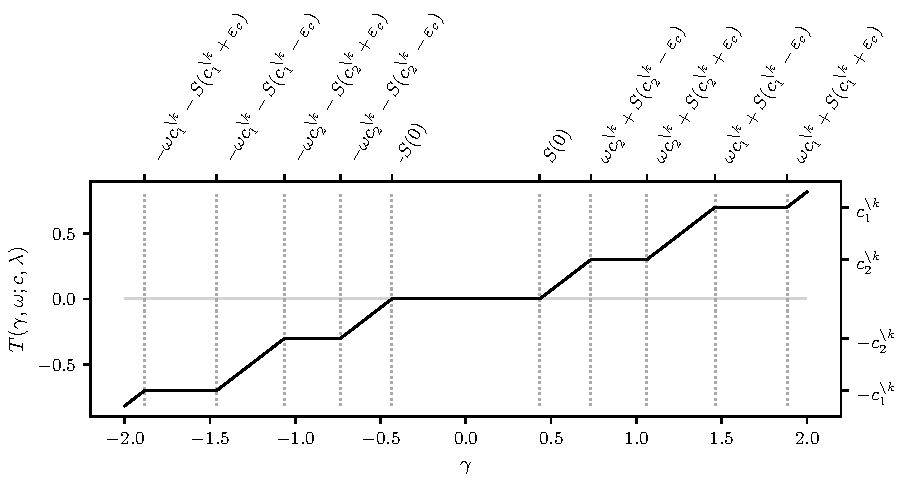
\includegraphics[width=\natwidth]{images/slope-thresholding.pdf}
  \caption{%
  The SLOPE thresholding operator. We define
  \(S(x) = \sum_{j \in C(x)}\lambda_{(j)^-_{x}}\)
  }
  \label{fig:slope-thresholding}
\end{figure}

The hybrid nature of the algorithm comes with boons of its own.
Indeed, proximal gradient descent algorithms are known to converge under
more general assumptions than coordinate descent algorithms. In effect,
this means that the PGD steps act as a safeguard and fallback
when coordinate descent struggles to converge.

One might imagine that this approach of hybrid algorithms could be
extended to standard Newton methods as well and, moreover, include more
refined heuristics in order to adapt naturally to problem structure.
This, however, is beyond the scope of our current work.

In addition to the implementation from \citet{larsson2023}, we have also
implemented a randomized\footnote{Using random permutations.} version
of the algorithm, which we have found to be more robust to numerical issues (at the
cost of slightly slower convergence).

Regarding updates of the intercepts, if we are in a PGD step, then the
intercept is updated as part of the full gradient step. If we are in a
coordinate descent step, then we can compute the intercept update at the end of
a full pass over the clusters.

\subsection{Convergence criteria}

Our packages use a duality-based stopping criterion, providing an upper bound
on suboptimality at convergence. We transform the primal problem into a
constrained formulation and derive a dual problem that allows us to compute a
duality gap. As a stopping criterion, we use the relative duality gap: \[
  P(\beta_0, \beta) - D(\delta) \leq \varepsilon | P(\beta_0, \beta) |, \] where
\(\varepsilon >0\) is the user-defined tolerance level. This provides a
reliable, solver-independent measure of convergence. The complete derivation of
the dual problem and the calculation of the duality gap is provided in
\Cref{sec:convergence-criteria-details}.

\subsection{Path fitting}

Our packages are optimized for fitting the full regularization path for SLOPE, which
is the sequence of solutions to the problem in \Cref{eq:slope} as \(\alpha\) is varied
from \(\alpha_\text{max}\), at which point the first cluster enters the model,
to a small value of \(\alpha\) at which the model is almost saturated.
We use the same criteria as \citet{friedman2010} for stopping the path early,
except that we stop if the number of \emph{clusters} excluding the zero-cluster
exceeds \(n + 1\) (by default), since the support of SLOPE is limited at \(n\) clusters,
which can potentially exceed the number of non-zero coefficients.\footnote{In practice
  this is quite rare since clusters do not form easily at low levels of regularization.}

Since an optimal setting for \(\lambda\) is only available under
strict assumptions that are typically hard to test, it

\subsection{Screening rules and working sets}

Sparse models, like lasso, SCAD, MCP, and SLOPE, benefit greatly from
so-called \emph{screening rules}, which are used to reduce the dimension of
\(\beta\) in the optimization problem. The basic intuition for this is that
it is possible to estimate the gradient \(\nabla F(\beta) \) for a given SLOPE problem
and use this to determine, via the subdifferential, which coefficients are
likely to be non-zero. This screening rule can either be heuristic or safe:
in the latter case the rule guarantees that excluded features correspond
to zero coefficients in the final model. Heuristic rules, on the other hand,
do not guarantee this and therefore need to be complemented with a pass
over all coefficients at the end to ensure that the optimality conditions
are satisfied. Since they are less conservative, however, the cost of
doing so is typically outweighed by the savings in computation time.
Heuristic and safe rules can be combined, usually at no extra cost since
they both rely on the same gradient information.

In the SLOPE package, we use the strong screening rule for
SLOPE~\citep{larsson2020a}, which is an extension of the working set strategy
for the strong screening rule for the lasso~\citep{tibshirani2012}.

\subsection{Covariance updates}

\citet{friedman2010} present an alternative coordinate descent update that is
based on pre-computing the Gram matrix \(X^\intercal X\) and then use this to
speed up the updates. As the authors note, this can lead to dramatic speed-ups
for the ordinary lasso (with least-squares loss), but not for other loss
functions and not in the high-dimensional setting.

Yet, although this type of update would be useful for SLOPE as well, it is not
implemented in our packages. The main reason for this is that the Gram matrix
we need is the collapsed version \((XP)^\intercal XP\), where \(P\) is the
pattern matrix, which cannot be derived from \(X^\intercal X\). \(P\) typically
changes continuously throughout optimization, which means that the precomputed
Gram matrix must be updated as well, and this would invoke additional cost.

\section{Implementation details}
\label{sec:implementation-details}

\subsection{Clusters}
\label{sec:clusters}

Handling the cluster structure of SLOPE is a key part of the algorithm since we
will both be iterating over the clusters as part of the coordinate descent
updates as well as updating the clusters after each update. In our
implementation, we represent the clusters as a collection of three vectors:

\begin{description}
  \item[\code{c}] The coefficients of the clusters
  \item[\code{c\_idx}] Pointers to the coefficients in the cluster
  \item[\code{c\_ptr}] Values of the cluster pointers
\end{description}

In this representation, the indices for the \(k\)th cluster are given by \code{
c_idx[c_ptr[k] : c_ptr[k+1]]} and the coefficient is simply \code{c[k]}.

This structure is the same basic setup as in \citet{larsson2023}. Unlike
their implementation, however, we have made improvements to the
handling of updating the clusters (merging,
reordering, removal), which can now be performed with negligible
overhead and with minimal copying.

Our representation of clusters closely resembles the sparse matrix
representation of the SLOPE pattern~\citep{schneider2022}. \(P\) is the pattern
matrix, \(X P\) is the collapsed design matrix. \(P\) contains only
zeros and signed ones. This means that we can obtain \(\tilde{x}\) in
\Cref{alg:hybrid} by multiplying the design matrix \(X\) with
a column of \(P\).

\subsection{Thresholding operator}

The SLOPE thresholding operator is the analogue to the
soft-thresholding operator for the lasso. But unlike the
latter, which is trivial to compute, the SLOPE thresholding operator
needs to conduct a search over the clusters in order to find correct
solution. This leads to a worst-case complexity of
\(\mathcal{O}(K)\), which could be prohibitive in practice.
Fortunately, the situation is much less dire in practice, since
the order of the clusters typically stabilizes early. Instead, the
bulk of the computational time is spent on computing the gradient.
For this reason we use a linear search, which, although suboptimal
theoretically, is faster than a binary search in practice.

We have, however, improved the implementation of
operator by \citet{larsson2023} significantly. In their implementation,
partial \(\lambda\) sums were in each iteration of the search, which
for some cases could lead to large overhead when updating
a large cluster. In our implementation, we instead use a lazy
evaluation strategy based on the cumulative sum of the \(\lambda\) array,
which causes no additional overhead.

\subsection{Sparsity}

Our package is based on the Eigen C++ library and works naturally with sparse
design matrices. These can be created directly through the
\pkg{Matrix}~(\proglang{R}), \pkg{scipy}~(\proglang{Python}), and \pkg{SparseArrays}~(\proglang{Julia}) packages in
and can be passed directly to the C++ API with negligible overhead
and without copying. Coefficients are returned in a sparse format, which
allows for efficient storage and retrieval of the coefficients.

\subsection{Parallelization}

The software is parallelized using OpenMP, which is supported
on all major platforms\footnote{Although overhead for creating
  multiple threads is considerably more demanding on Windows}.
Functions make use of heuristics to determine whether to
spawn multiple threads depending on problem size, except for
the embarassingly parallel case of cross-validation, which is always
parallelized.

\subsection{Feature normalization}

As shown by \citet{larsson2025}, feature normalization (centering and
scaling the design matrix) can have large consequences for the
solutions. In our packages, we provide multiple different options
for centering and scaling, independently of one another.
We also provide the possibility to manually supply centering
and scaling vectors.

We have also implemented just-in-time (JIT) normalization, which
means that the design matrix does not need to be normalized
in advance. Instead, normalization is performed on-the-fly during
optimization, which means that we can allow arbitrary centering
even of sparse design matrices. In addition, we can completely
avoid copying the design matrix.

\subsection{Memory management}
\label{sec:memory-management}

For dense matrices, the packages implement memory-efficient views of
the input matrices in order to avoid copies of the data.\footnote{This is technically achievable for sparse matrices too, but
  would mean heavy overhead since we would need to iterate over all nonzero
  elements for each view. We have thus decided against implementing this.}
This means, for instance, that no copies need to be made when separating
data sets into training and test data.

\subsection{Cross-validation}

Due to the memory-efficient implementation of view~\Cref{sec:memory-management}, we provide
an option to altogether avoid copying the data during cross-validation.
This means that we parallelize the cross-validation procedure over
arbitrarily many folds and repetitions, yet still completely
avoid the need to copy the data.

\subsection{Out-of-memory support}

The SLOPE packages support out-of-memory storage for the design matrix, which
means that users can fit SLOPE models on data sets that are larger than the
available memory. Storage in RAM is therefore limited to the order of \(O(n) +
O(p)\), which means that the packages can be used on huge data sets.

This is supported via the generic \code{Eigen::Map} class, which allows
arbitrary data to be mapped into \pkg{Eigen} data structures. At the
time of writing, this is only supported for \proglang{R},
which is possible via the \pkg{bigmemory} package~\citep{kane2013},
and currently only for dense designs.

\subsection{Software}
\label{sec:implementation}

In this paper we present a collection of packages for solving SLOPE, currently
with support for fitting SLOPE in \proglang{R}, \proglang{Python}, and
\proglang{Julia}. The backbone of all of these packages is based on a
\proglang{C++} library that implements all of the numerical algorithms for
SLOPE, including preprocessing, cross-validation, and path fitting. The
packages for the high-level languages all serve as thin wrappers to the
\proglang{C++} library, with some additional functionality for handling data
and plotting the results. This means that new features and bug fixes propagate
quickly and easily to all these wrapppers and enable users to promptly take
advantage of the latest developments.

The entire suite of packages is open source and licensed under the GPL-3.0 license,
and is available on GitHub~(\Cref{tab:slope-packages}).

\begin{table}[t!]
  \centering
  \begin{tabular}{llll}
    \toprule
    Language          & Package        & Repository                         & Documentation                     \\
    \midrule
    \proglang{R}      & \pkg{SLOPE}    & \myurl{github.com/jolars/SLOPE}    & \myurl{jolars.github.io/libslope} \\
    \proglang{Python} & \pkg{sortedl1} & \myurl{github.com/jolars/sortedl1} & \myurl{jolars.github.io/sortedl1} \\
    \proglang{Julia}  & \pkg{SLOPE.jl} & \myurl{github.com/jolars/SLOPE.jl} & \myurl{jolars.github.io/SLOPE.jl} \\
    \proglang{C++}    & \pkg{slope}    & \myurl{github.com/jolars/libslope} & \myurl{jolars.github.io/libslope} \\
    \bottomrule
  \end{tabular}
  \caption{SLOPE packages}
  \label{tab:slope-packages}
\end{table}

This is made possible via several pieces of software that enable us to link the
API from our \proglang{C++} library to the high-level languages. This includes
\pkg{Rcpp}~\citep{eddelbuettel2011} and \pkg{RcppEigen}~\citep{bates2013} for
\proglang{R}, \pkg{pybind11}~\citep{jakob2025}, and \pkg{CxxWrap}~\citep{janssens2020} for
\proglang{Julia}.

\section{Examples}

In this section we will show how to use the packages to fit SLOPE models in
the different languages.

The packages are
available through the respective package managers for each language, and can be
be installed using the following commands:

\begin{description}[labelwidth=8ex]
  \item[\proglang{R}] \code{R> install.packages("SLOPE")}
  \item[\proglang{Python}] \code{$ pip install sortedl1}
  \item[\proglang{Julia}] \code{julia> using Pkg; Pkg.add("SLOPE")}
\end{description}

Installing the \proglang{C++} library is slightly more involved, and requires
\pkg{CMake}~\citep{kitware2025} together with a working \proglang{C++} toolchain, including
the \pkg{Eigen} library~\citep{guennebaud2010a} and \pkg{OpenMP}~\citep{dagum1998}.

Assuming that we have loaded a data set consisting of a design
matrix \code{x} and response vector \code{y}, we can fit the full regularization
path for the SLOPE model using the following commands for the different languages:

\begin{minipage}[t]{0.25\textwidth}%
  \textbf{\proglang{R}}
  \begin{Code}
R> library(SLOPE)
R> fit <- SLOPE(x, y)
  \end{Code}
\end{minipage}
\hfill
\begin{minipage}[t]{0.32\textwidth}

  \textbf{\proglang{Python}}
  \begin{Code}
>>> import sortedl1
>>> model = sorted1.Slope()
>>> res = model.path(x, y)
  \end{Code}
\end{minipage}
\hfill
\begin{minipage}[t]{0.32\textwidth}
  \textbf{\proglang{Julia}}
  \begin{Code}
julia> using SLOPE
julia> fit = slope(x, y)
  \end{Code}
\end{minipage}

\medskip

You can also use the C++ library directly, in
which case the above would translate into the
following:
\begin{Code}
#include <slope/slope.h>
slope::Slope model;
auto path_result = model.path(x, y);
\end{Code}

In the sequel, we will focus our examples on the \proglang{R} package, but
note that the API is very similar in all of the languages.

\subsection{First steps}

We start with a simple example of fitting a full SLOPE path to the diabetes
data set~\citep{efron2004}, including plotting it.

\begin{Code}
R> library(SLOPE)
R> data("diabetes", package = "lars")
R> x <- scale(diabetes$x)
R> y <- diabetes$y
R> fit_slope <- SLOPE(x, y, q = 0.1)
R> plot(fit_slope)
\end{Code}

The \code{q} parameter is a parameter of the sequence of \(\lambda\) values,
which by default~(\code{lambda = "bh"}) is the Benjamini--Hochberg (BH)
sequence~\citep{bogdan2015}. If the design matrix is orthogonal, then the
\code{q} parameter will decide the expected false discovery rate (FDR) in terms
of the identification of true signals (nonzero coefficients), provided
that this sequence is used.

Other types of sequences are also supported,
including \code{lambda = "lasso"} for the lasso
\code{lambda = "oscar"} for the OSCAR sequence~\citep{bondell2008}, and
\code{lambda = "gaussian"} for the Gaussian-type sequence~\citep{bogdan2015},
which is a modification of the BH sequence that has been empirically shown to
provide similar FDR control in non-orthogonal and low-dimensional settings.

To show how the choice of the \(\lambda\) sequence affects the
results, we will refit the diabetes data using the lasso sequence.

\begin{Code}
R> fit_lasso <- SLOPE(x, y, lambda = "lasso")
R> plot(fit_lasso)
\end{Code}

The resulting paths are plotted in \Cref{fig:diabetes}. Observe that the
paths are overall similar but that the SLOPE path has clustered
some coefficients for parts of the path. Predictors 3 and 9, for instance,
enter the path together and remain clustered at the beginning, then
split apart and again cluster together briefly, before diverging again.
We also see that predictor 6 joins the path briefly together
with predictor 5 on the SLOPE path, but then return to zero until
it later enters again on its own.

\begin{figure}[t]
  \centering
  {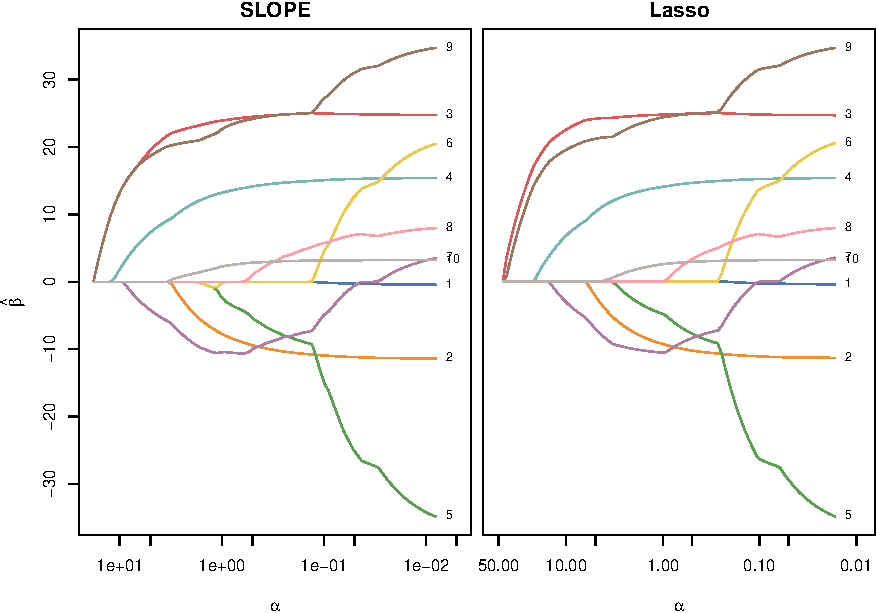
\includegraphics[width=\natwidth]{images/diabetes-slope-lasso.pdf}}
  \caption{%
    SLOPE and lasso paths on the diabetes
    data set.
  }
  \label{fig:diabetes}
\end{figure}

% TODO: We first need to implement this in the package.

\subsection{Relaxed SLOPE}

Unlike the lasso, the relaxed version of SLOPE has not been studied in much detail.
There are at least two papers where it is described, but then typically it is
called \emph{debiased} SLOPE. We prefer to use the term \emph{relaxed} here,
since it corresponds closer to the terminology from the lasso literature and
avoids confusion with the debiased lasso~\citep{geer2014}, which is a different
model.

In our packages, we support the relaxed version of SLOPE, and parameterize
this relaxation with a parameter \(\gamma\).

The relaxation parameter \(\gamma\) controls the mix between the
original SLOPE solution (\(\gamma = 1\) and the fully relaxed
solution (\(\gamma = 0\)), so that
the end result is given by
\[
  \hat{\beta} = \gamma \hat{\beta}_\text{SLOPE} + (1 - \gamma) \hat{\beta}_\text{relaxed}.
\]

Here, we fit two models, one that is fully relaxed
(\(\gamma = 0\)) and one that is semi-relaxed (\(\gamma = 0.5\)).

\begin{Code}
R> fit_relaxed <- SLOPE(x, y, q = 0.1, gamma = 0)
R> fit_semirelaxed <- SLOPE(x, y, q = 0.1, gamma = 0.5)
\end{Code}

We fit the result in \Cref{fig:relaxed-slope}.

\begin{figure}[t]
  \centering
  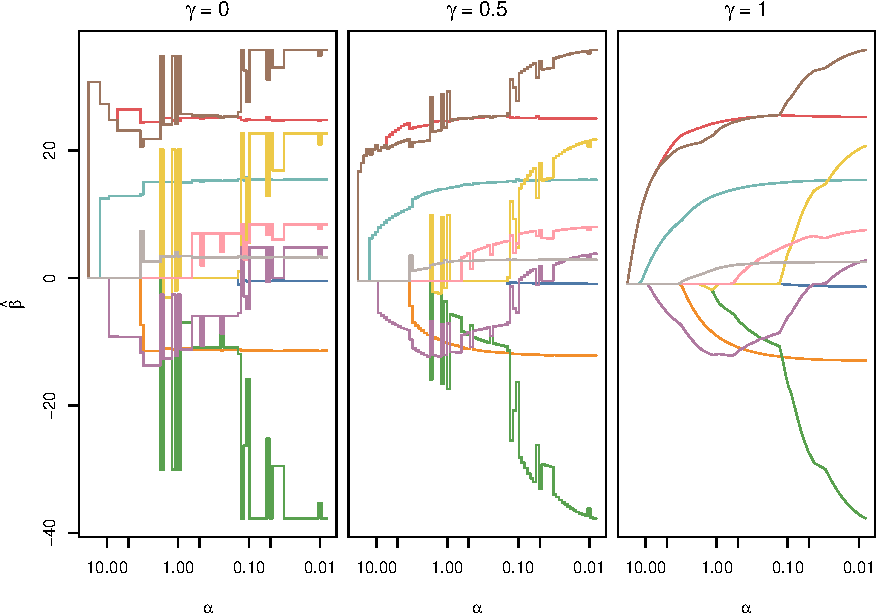
\includegraphics[width=\natwidth]{images/slope-relaxed.pdf}
  \caption{%
    SLOPE with various level of relaxation \(\gamma\), with
    \(\gamma = 0\) (fully relaxed), \(\gamma = 0.5\) (semi-relaxed),
    and \(\gamma = 1\) (standard SLOPE).
  }
  \label{fig:relaxed-slope}
\end{figure}

\subsection{Cross-validation}

Our packages support hyper-parameter tuning via iterated \(k\)-fold
cross-validation, with parameterization over \(\alpha\), \(\lambda\) type (BH,
Gaussian type, etc.), \(\gamma\) (SLOPE relaxation parameter).

Here, we show the CV functionality by cross-validating across
to values of the \(q\) parameter.

\begin{CodeChunk}
  \begin{CodeInput}
R> set.seed(48)
R> fit_cv <- cvSLOPE(x, y, q = c(0.1, 0.2))
R> plot(fit_cv)
\end{CodeInput}
  \begin{CodeOutput}
Call:
cvSLOPE(x = x, y = y, q = c(0.1, 0.2))

Optimum values:
      q gamma     alpha measure     mean       se      lo       hi
129 0.2     0 0.3379402     mse 3013.065 234.6321 2482.29 3543.839
\end{CodeOutput}
\end{CodeChunk}

It is also easy to plot the cross-validation results~\Cref{fig:cv}.

\begin{Code}
R> plot(fit_cv)
\end{Code}

\begin{figure}[t]
  \centering
  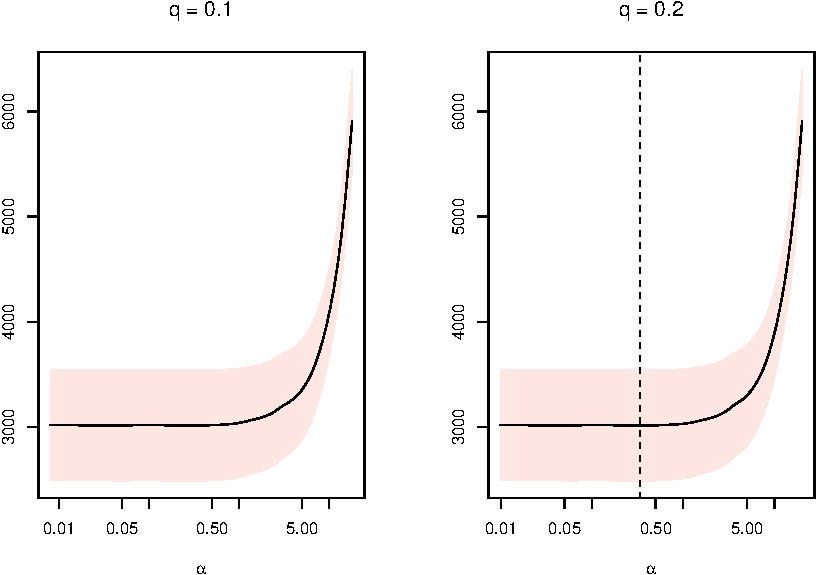
\includegraphics[width=\natwidth]{images/slope-cv.pdf}
  \caption{%
    Mean-squared error (MSE) from cross-validation of
    \(q\) and \(\alpha\) for SLOPE fit to the diabetes data set.
    The dashed line marks the optimal value of \(\alpha\) in the
    panel corresponding to the optimal value of \(q\).
  }
  \label{fig:cv}
\end{figure}

It is also possible to cross-validate over the \(\gamma\) parameter, to
find the optimal level of relaxation for SLOPE.

\section{Benchmarks}

\citet{larsson2023} developed a benchmark for SLOPE using
\pkg{benchopt}~\citep{moreau2022a}: a command-line interface and Python library
for creating and managing benchmarks of algorithms for optimization. As part of
our work, we have extended this benchmark to include additional solvers. The
benchmark for SLOPE is available at
\myurl{github.com/benchopt/benchmark\_slope}, which featres the
\proglang{Python} implementation of SLOPE, \pkg{sortedl1}, as well as the
\proglang{R} implementation, \pkg{SLOPE}.

For this paper, we have run the benchmarks for some real data sets~\Cref{tab:real-data},
as well as simulated data\Cref{tab:simulated-data}.

\begin{table}[hbt]
  \centering
  \label{tab:real-data}
  \begin{tabular}{
      l
      S[table-format=5.0]
      S[table-format=7.0]
      S[table-format=1.5,round-mode=figures,round-precision=2]
      p{5cm}
    }
    \toprule
    Dataset                    & {\(n\)} & {\(p\)} & {\(X\) density} & {References}                        \\
    \midrule
    \dataset{Koussounadis2014} & 101     & 34694   & 1               & \citet{koussounadis2014}            \\
    \dataset{brca1}            & 536     & 17322   & 1               & \citet{nationalcancerinstitute2022} \\
    \dataset{news20}           & 19996   & 1355191 & 0.0003357       & \citet{keerthi2005}                 \\
    \dataset{rcv1}             & 20242   & 44504   & 0.00166         & \citet{lewis2004}                   \\
    \dataset{Rhee2006}         & 842     & 360     & 0.02469         & \citet{rhee2006}                    \\
    \bottomrule
  \end{tabular}
  \caption{%
    List of real datasets used in our experiments.
    x were obtained from \citet{breheny2022}  and the rest from \citet{chang2016}.
  }
\end{table}

\begin{table}[t]
  \centering
  \label{tab:simulated-data}
  \begin{tabular}{
      l
      S[table-format=5.0]
      S[table-format=7.0]
      S[table-format=2.0]
      S[table-format=1.3]
      S[table-format=0.1]
    }
    \toprule
    {Scenario} & {\(n\)} & {\(p\)} & {\(k\)} & {\(X\) density} & {\(\rho\)} \\
    \midrule
    1          & 200     & 20000   & 20      & 1               & 0.6        \\
    3          & 200     & 200000  & 20      & 0.001           & 0.6        \\
    2          & 20000   & 200     & 40      & 1               & 0.6        \\
    \bottomrule
  \end{tabular}
  \caption{Scenarios for the simulated data in our benchmarks}
\end{table}

\begin{description}
  \item[sortedl1] The python package of our implementation of the hybrid
        proximal gradient/coordinate descent algorithm described in this work and
        \citet{larsson2023}.
  \item[PGD] The proximal gradient descent algorithm, which is a standard
        algorithm for solving convex optimization problems~\citep{wright2009}. We use a
        analytical computation of the Lipschitz constant to pick the step size.
  \item[PGD-Anderson] The PGD algorithm with Anderson acceleration, which is a
        method for accelerating the convergence of fixed-point
        iterations~\citep{anderson1965,zhang2020}.
  \item[PGD-BB] The PGD algorithm with Barizilai--Borwein~\citep{barzilai1988} step sizes.
  \item[PGD-Safe] A PGD-based algorithm using safe screening rules~\citep{elvira2023}.
  \item[FISTA] An accelerated version of PGD~\citep{beck2009}.
  \item[ADMM] The alternating direction method of
        multipliers~\citep{glowinski1975,boyd2010}, which is a popular algorithm
        for solving convex optimization problems with constraints.
  \item[Newt-ALM] A semi-smooth Newton-based method~\citep{luo2019}. We use the
        implementation of this method from \citet{larsson2023}.
  \item[skglm] Another implementation of FISTA, but with working sets, from the
        \pkg{skglm} package~\citep{bertrand2022}.
  \item[SlopePath] An approximate homotopy method by \citet{dupuis2024},
        which is similar to the lars algorithm for the lasso~\citep{efron2004}.
\end{description}

\begin{figure}[t]
  \centering
  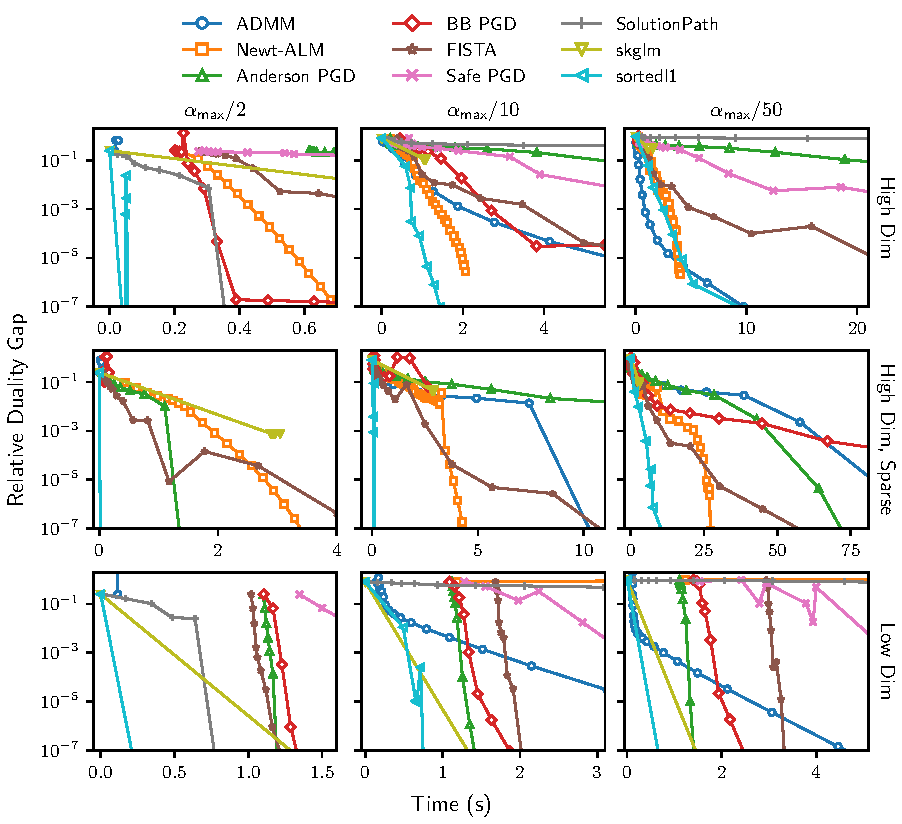
\includegraphics[width=\natwidth]{images/benchmark_single_simulated.pdf}
  \caption{%
  }
  \label{fig:simulated-data-single}
\end{figure}

\begin{figure}[tp]
  \centering
  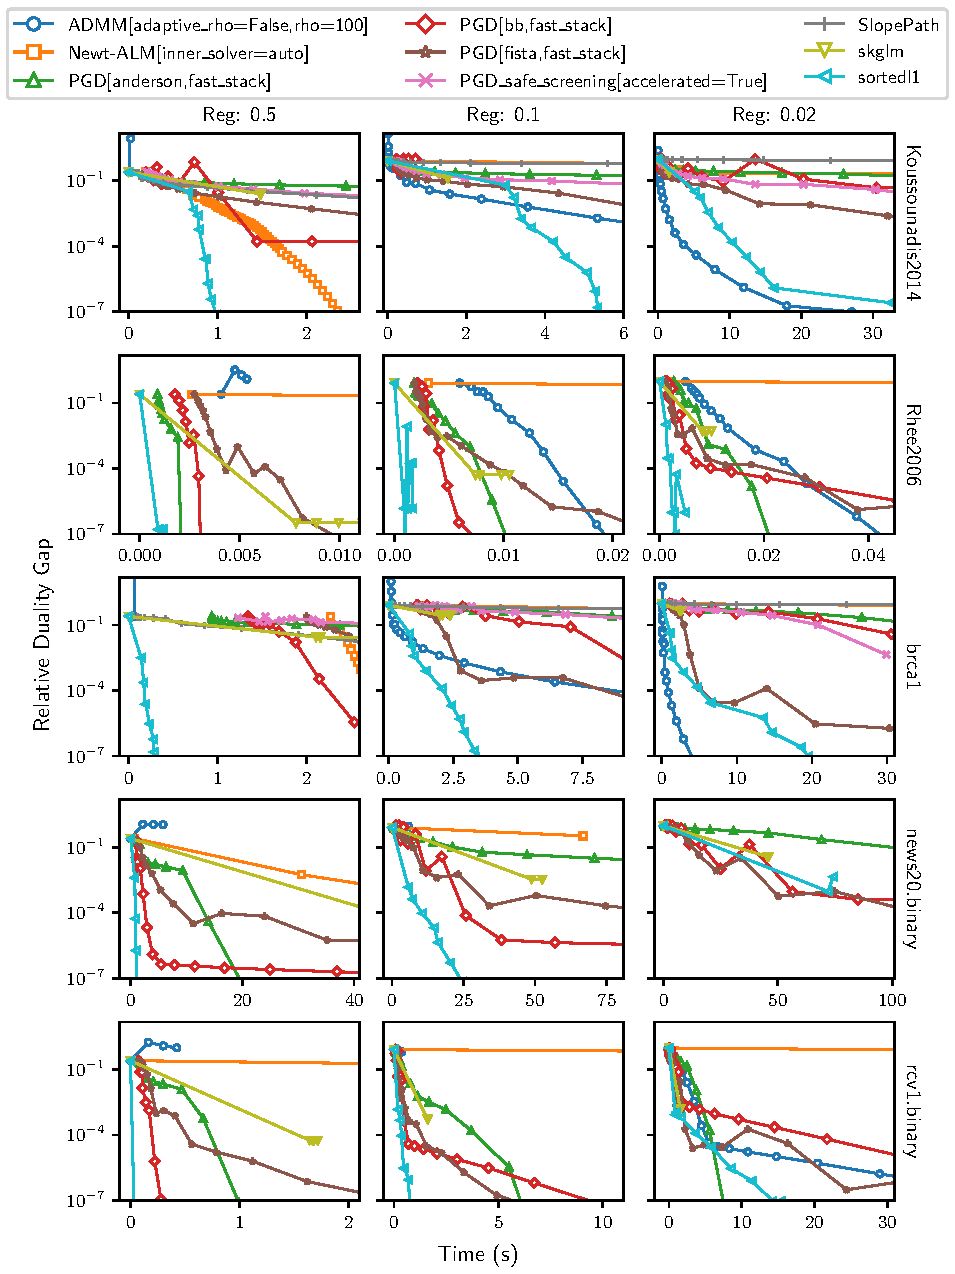
\includegraphics[width=\natwidth]{images/benchmark_single_real.pdf}
  \caption{%
  }
  % \label{fig:real-data-single}
\end{figure}

We have also created a separate benchmark for fitting the full regularization
path, which is available at \myurl{github.com/benchopt/benchmark\_slope\_path}.
Here, we present benchmarks on a subset of the real data sets
from \Cref{tab:real-data}. We parameterize the benchmark using
the lenth of the path, using 50, 100, and 200 steps. We present the results
as the maximum relative duality gap along the path.

The results are presented in \Cref{fig:real-data-path}. Note the interpretation
as progress towards convergence does not hold quite the same way as for the single
solution benchmarks since we fit a full path. Nevertheless, we note that our
implementation is the fastest by a large margin.

\begin{figure}[t]
  \centering
  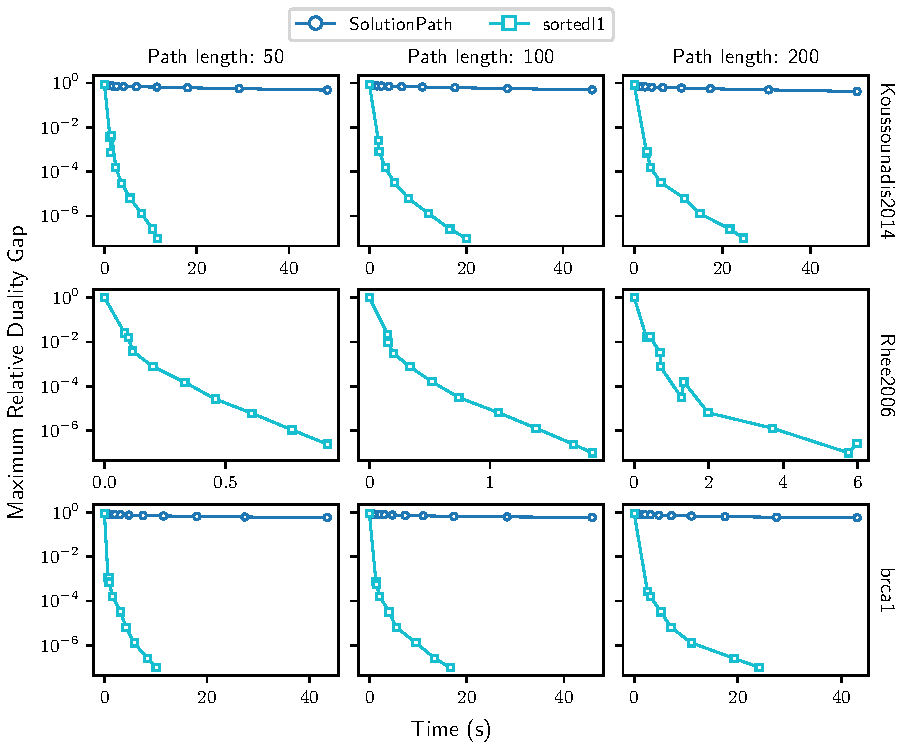
\includegraphics[width=\natwidth]{images/benchmark_path_real.pdf}
  \caption{%
    Benchmark for fitting the full regularization path on real data sets.
  }
  \label{fig:real-data-path}
\end{figure}

\section{Discussion}

SLOPE is an appealing model for high-dimensional regression problems that is
able to provide sparse solutions with a cluster structure, which sets it apart
from similar models such as the lasso and elastic net. Unlike these models,
however, SLOPE represents a more challenging optimization problem since the
penalty term is inseparable. In spite of this, we have shown that it is
possible to solve SLOPE efficiently and have, in paper, presented a collection
of packages (in \proglang{R}, \proglang{Python}, and \proglang{Julia}) that do
so. In so doing, we hope to have made SLOPE accessible to a wider audience.
Ours are the first packages that implement SLOPE in these languages and
are still unmatched in terms of features. We know only of one other
implementation of SLOPE in \proglang{Python}, and none in \proglang{Julia} and
\proglang{R}.

We have shown that the performance of our software is unparalleled
compared to other algorithms and implementations, both for for fitting
the full regularization path as well as for single solution, and
have shown these in a series of benchmarks on both real and simulated
data. We have also made these benchmarks available publicly
to facilitate further research and development of SLOPE.

\citet{dupuis2024} benchmarked the Python implementation of the hybrid
algorithm from \citet{larsson2023} against their approximate homotopy method
and showed that their method performed better in certain cases. We have not
seen this result in our benchmarks even when fitting the full regularization path.
Besides the fact that the current implementation of our algorithm
is more efficient than the one from \citet{larsson2023}, we believe that
this may also be due to the smaller problem sizes in \citet{dupuis2024}'s
work as well as the fact that they compared times at convergence to
a duality gpa of \(10^{-10}\), which is more stringent than our results.

Although our packages are full-fledged implementations of SLOPE, there are
still some features that are missing. For instance, we do not yet support
observation weights, nor some of the more advanced features of similar packages
such as \pkg{glmnet}~\citep{friedman2010}, which allow for a larger variety of
loss functions, including Cox proportional hazards models and multivariate
linear regression. We also do not yet support the group sorted \(\ell_1\) norm,
which would allow an alternative penalization scheme for multivariate response
problems. In addition, several possible improvements to the hybrid method
could be considered, such as accelerated and parallelized coordinate
steps. We leave these as future work, but note that
the packages are modular and have been designed with extensibility in mind,
which we hope will facilitate the addition of new features in the future.
Because all of the packages rely on the same \proglang{C++} library, contributions
will propagate quickly to all of the packages.

We hope that our packages will be useful for researchers and
practitioners alike and that the design of our software suite
might inspire others to more closely couple the available features
of \proglang{R}, \proglang{Python}, and \proglang{Julia} and avoid
redundant implementations of the same algorithms in each language.

\bibliography{main}

\newpage

\begin{appendix}

  \section{Duality gap and convergence criteria}
  \label{sec:convergence-criteria-details}

  In detail, we transform the primal problem \(P\), defined in \Cref{eq:slope}, into a
  constrained problem, taking \(\alpha = 1\) without loss of generality:
  \begin{equation}
    \label{eq:slope-constrained}
    \begin{aligned}
       & \minimize_{\beta_0 \in \mathbb{R},\beta \in \mathbb{R}^p} &  & \frac{1}{n} \sum_{i=1}^n f(y_i, x_i^\intercal \beta + \beta_0) + J_{\lambda}(\beta) \\
      % & \text{subject to}                                              &  & r_i = \link(\bm{x}_i^\intercal \bm{\beta}) - y_i, \quad i = 1, \ldots, n                                            \\
       & \text{subject to}                                         &  & r_i = \ilink(\beta_0 + x_i^\intercal \beta) - y_i, \quad i = 1, \ldots, n           \\
    \end{aligned}
  \end{equation}

  Since \(\beta_0 + x_i^\intercal \beta = g(r_i + y_i)\), we can write the Lagrangian as
  \[
    L(\beta_0,\beta,r,\delta) = \frac{1}{n} \sum_{i=1}^n f\big(y_i, g(r_i + y_i)\big) + J_{\lambda}(\beta) - \sum_{i=1}^n \delta_i \left(g(r_i + y_i) - x_i^\intercal \beta - \beta_0 \right).
  \]
  This allows us to write the dual problem as
  \[
    D(\delta)  = \inf_r\left( \frac{1}{n} \sum_{i=1}^n f\left(y_i, g(r_i+y_i)\right) - \delta_i g(r_i+ y_i)\right)
    % & \phantom{={}} + \inf_\beta \left(J_\lambda(\beta) - \delta^\intercal X\beta\right)   \\
    % & \phantom{={}} + \inf_{\beta_0} \left( -\delta^\intercal \bm{1} \beta_0\right)        \\
    - \sup_\beta \big((-X^\intercal \delta)^\intercal \beta -  J_\lambda(\beta) \big)
    - \sup_{\beta_0} \left( \delta^\intercal \bm{1} \beta_0\right).
  \]
  Here, we begin by noting that the infimum is attained at the point where
  \(r = \delta\)~\citep{fercoq2015}, which means that the value is
  \[
    \frac{1}{n} \sum_{i=1}^n f\left(y_i, g(\delta_i+y_i)\right) - \delta_i g(\delta_i + y_i)
  \]
  in general, although loss-specific simplifications can be made. For instance, in the case of
  quadratic loss the expression evaluates to \(\frac{1}{2} \lVert y \rVert_2^2 - \frac{1}{2} \lVert \delta + y \lVert^2_2 \).

  Next, we observe that \(\sup_\beta \big((-X^\intercal
  \delta)^\intercal \beta -  J_\lambda(\beta) \big)\) is the Fenchel conjugate of
  the sorted \(\ell_1\) norm, which is the indicator function of the sorted
  \(\ell_1\) dual norm unit ball. Its value is
  \[
    \sup_\beta \big(z^\intercal \beta -  J_\lambda(\beta) \big) =
    \begin{cases}
      0      & \text{if } J^*_\lambda(z) \leq 1, \\
      \infty & \text{otherwise},
    \end{cases}
  \]
  where \(J^*_\lambda(z)\) is the sorted \(\ell_1\) dual norm, defined as~\citep{negrinho2014}
  \begin{equation}
    J^*_\lambda(z) = \max_{j=1,2,\dots,p}\left\{ \frac{\sum_{k=1}^j|z_{(k)}|}{\sum_{k=1}^j\lambda_k}\right\}
  \end{equation}

  Next, observe that \(\sup_{\beta_0} (\delta^\intercal \bm{1} \beta_0) = \infty\) unless
  \(\delta^\intercal \bm{1} = 0\).

  Taken together, this means that we have the following dual function:
  \begin{equation}
    D(\delta) = \begin{cases}
      \frac{1}{n} \sum_{i=1}^n f\left(y_i, g(\delta_i+y_i)\right) - \delta_i g(\delta_i+ y_i) & \text{if } J^*_\lambda(-X^\intercal \delta) \leq 1 \text{ and } \delta^\intercal \bm{1} = 0 \\
      -\infty,                                                                                & \text{otherwise}.
    \end{cases}
  \end{equation}

  A natural dual point candidate for this problem is to pick
  \(\delta = r\), since
  at the optimum we have
  \[
    \bm{0} \in X^\intercal r + \partial J_\lambda(X^\intercal r)
  \]
  and, in addition require that the signs between agree.
  % TODO: Hand-wavy, clean up later.

  % To obtain a feasible dual point for this problem, we can use the
  % following fact about the stationarity condition of the primal problem,
  % namely that
  % \[
  %   \sum_{j=1}^k | g_{(j)} | \leq \sum_{j=1}^k \lambda_j |\beta_{(j)}| \quad \forall\; k = 1,2,\dots,p.
  % \]
  % where  \(g_j = x_j^\intercal r\) is the \(j\)th component of the gradient of loss function
  % with respect to \(\beta_j\)
  % and \(r\) the generalized residual, for which \(r_i = \ilink(x_i^\intercal \beta + \beta_0) - y_i\).

  To be a feasible point, however, we first center the point by its mean and
  scale it:
  \[
    \delta_j = \frac{r_i - \bar{r}}{\max\left\{1, J_\lambda^*\left(X^\intercal(r - \bar{r})\right) \right\}}
  \]
  which guarantees feasibility. We then obtain the following duality gap:
  \[
    P(\beta_0, \beta) - D(\delta).
  \]
  As a stopping criterion for the algorithm, we use the relative duality gap
  \[
    P(\beta_0, \beta) - D(\delta) \leq \varepsilon P(\beta_0),
  \]
  where \(\varepsilon >0\) is the user-defined tolerance level.
  The duality gap provides an upper bound on suboptimality for the problem, independent
  of solver and conditioning of the problem, which is not the case of
  convergence criteria based on changes in objective, gradients, or coefficients.

  The availability of the duality gap would also allow us to employ
  duality-gap based safe screening rules~\citep{fercoq2015} and
  working set strategies derived from these~\citep{massias2018}, which
  could furthermore be used to enhance our strategy with look-ahead
  screening rules~\citep{larsson2021a}. However,
  as noted in \citet{larsson2022d}, the marginal improvement
  of using duality-based screening strategies is minor, so we have
  opted not to implement these in our packages.
  % TODO: Maybe reconsider this!

\end{appendix}

\end{document}
